For our chosen activation probability $p_A = 1/(j+2)$ it has been shown that aging is not able to modify the cascade condition from the original Threshold model. It is natural to ask about the generality of this result. In fact, in Fig. \ref{fig:exp_umbral} we show that for an exponential activation probability ($p_A = \exp{(-0.5(j+1))}$), the cascade condition is modified and the system does not reach the absorbing state for any values of the average degree $z$ and the threshold $T$ considered before (compare with Fig. \ref{fig:umbral}).

\begin{figure}[]
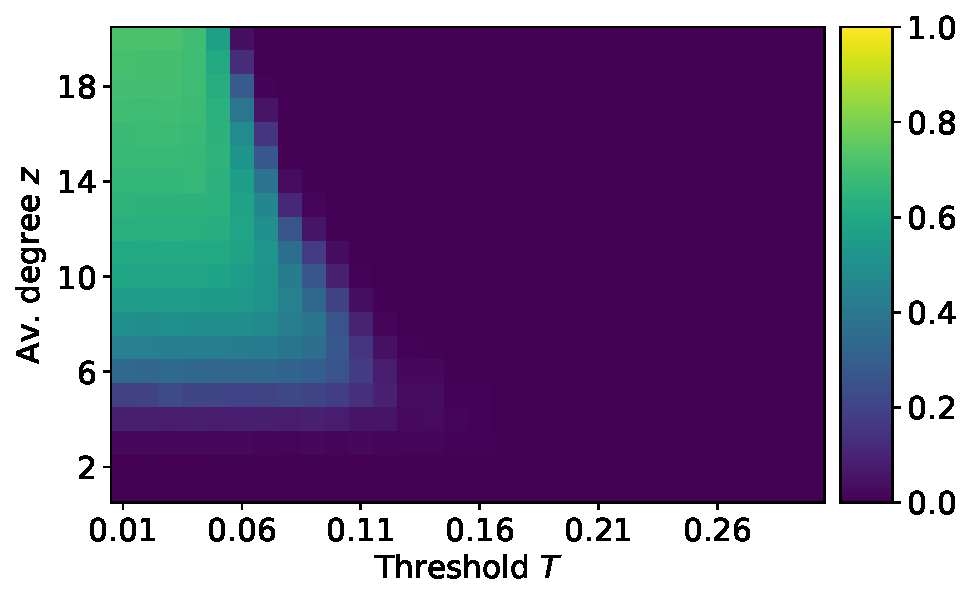
\includegraphics[width=1\columnwidth]{Figs/Appendix1_Threshold/cascade_exp.pdf}
\caption{\label{fig:exp_umbral} Average density $\rho$ of adopters for an Erd\H{o}s-R\'enyi graph of mean degree $z$ using the Symmetrical threshold model with endogenous aging with threshold $T$. The activation probability is exponential $p_A(j) = \exp{(-0.5*(j+1))}$. Color-coded values of $\rho$ are from Monte Carlo simulations of the model without aging in a graph with $N = 10,000$ agents.  Monte Carlo simulations are averaged over $M = 5 \times 10^4$ realizations.}
\end{figure}

One may think that this different behavior is because not all nodes are able to activate and adopt the technology with the exponential activation function. To clarify this issue, we computed the probability that an agent never activates during the whole evolution. Since we are performing a Random Asynchronous update in a network of size $N$, the probability that an agent is not activated in an update attempt is the probability of not being chosen plus the probability of being chosen and not activating:

\begin{align}
    Pr[\textrm{``agent is not activated in an attempt"}] = \nonumber \\
    \left(1 - \frac{1}{N}\right) + \frac{1}{N} (1 - p_{A}(j)).
\end{align}

As we are performing Monte-Carlo simulations, the probability of the agent being not activated after the $N$ update attempts of the Monte-Carlo step is:

\begin{align}
    Pr[\textrm{``agent is not activated in a MC step"}] = \nonumber \\
    \left[ \left(1 - \frac{1}{N}\right) + \frac{1}{N} (1 - p_{A}(j)) \right]^N.
\end{align}

Therefore, the probability that an agent is never activated is the probability that the agent does not get activated during the evolution, in other words, after infinite Monte-Carlo steps (where after each Monte-Carlo, since it has not been activated, the internal time $j$ increases by one):

\begin{align} \label{probability_never}
    Pr[\textrm{``agent is never activated"}] = \nonumber \\
    \prod_{j=0}^{\infty} \left[ \left(1 - \frac{1}{N}\right) + \frac{1}{N} (1 - p_{A}(j)) \right]^N.
\end{align}

For both activation probabilities, exponential ($p_A(j) = \exp{(-0.5(j+1))}$) and power law ($p_A(j) = 1/(j+2)$), following Eq. \eqref{probability_never}, the probability that an agent is never activated tends to $0$ for the long time simulation limit $j_{\rm max} \to \infty$ for any system size $N$. Therefore, all agents in the system activate at least once during the simulation. Thus, the reason that an exponential activation probability is able to change the cascade condition and a power law function is not just an activation effect, it is due to a non-trivial balance between activation and the adoption process. Notice that this calculation is the same for both aging mechanisms (endogenous and exogenous) because the difference between those appear after the first activation.